\chapter{Estado del Arte}

De la recopilaci\'on de antecedentes encontrados en la literatura, es posible separar los m\'etodos en dos categor\'ias. En la primera categor\'ia se encuentran enfoques asociados al an\'alisis de la reconstrucci\'on de filamentos en base a sus segmentos, como \cite{zhang2017extracting}, que identifica el problema de discontinuidad de filamentos en una imagen, pudiendo atribuirse esto a factores experimentales como la densidad del componente fluorescente, ruido u otras. Para llevar a cabo la reconstrucci\'on de un filamento en base a segmentos, establecen el uso de dos filtros, denominados \textit{Filtro de Transformaci\'on Lineal} (LFT por su sigla en ingl\'es) y \textit{Filtro de Transformaci\'on en base a la Orientaci\'on} (OFT por su sigla en ingl\'es). 
El filtro LFT busca resaltar caracter\'isticas lineales centr\'andose en cada p\'ixel y generando una serie de lineas con radio r, buscando la linea que contenga la mayor intensidad, seg\'un se observa en la figura \ref{fig:MTLFT}. El filtro OFT complementa lo anterior, mediante un criterio de similaridad en la direcci\'on proyectada de los segmentos, un criterio respecto a la distancia entre los extremos finales de cada segmentos y un criterio de continuidad, que limita el \'angulo entre vector proyectado de un extremo y el vector que representa la distancia entre los extremos de cada segmento. Lo anterior se puede observar en la figura \ref{fig:MTOFT}.

\begin{figure}[h]
        \centering
        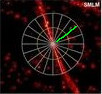
\includegraphics[scale=5]{imagenes/MT-LFT.jpeg}
        \caption{B\'usqueda por lineas con radio r para diferentes \'angulos, según filtro LFT. Fuente: \cite{zhang2017extracting}}
        \label{fig:MTLFT}
\end{figure}

\begin{figure}[h]
        \centering
        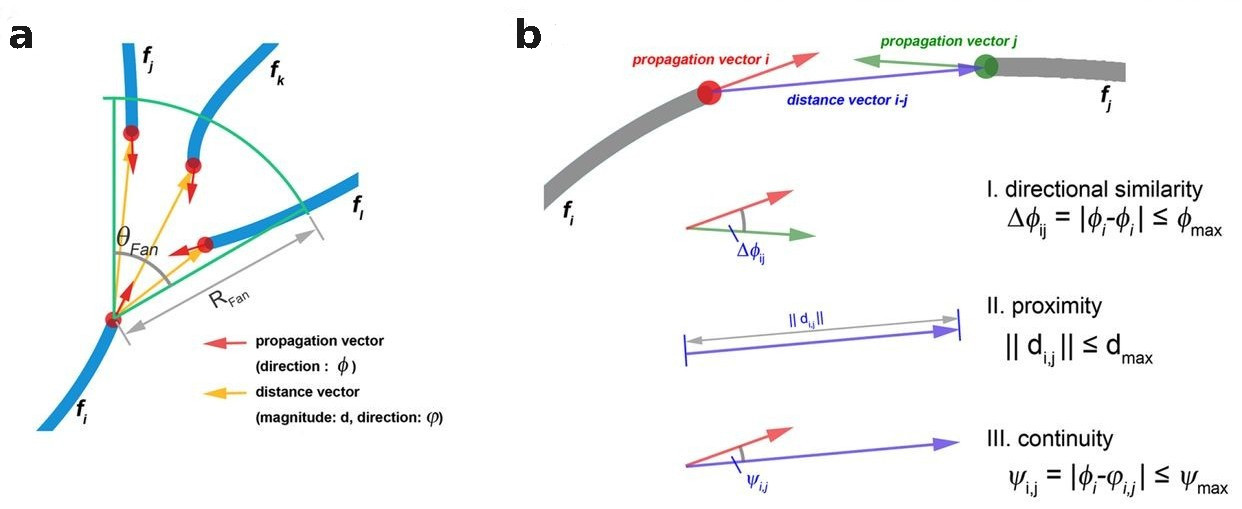
\includegraphics[scale=1.3]{imagenes/MT-OFT.jpeg}
        \caption{Criterios del filtro OFT: (A) Vectores de propagaci\'on (rojo) y distancia (amarillo) (B) Ejemplos de criterios de coincidencia de fragmentos de filamento I) Similaridad de direcci\'on, II) Proximidad, III) Continuidad. Fuente: \cite{zhang2017extracting}}
        \label{fig:MTOFT}
\end{figure}


El fundamento de los criterios de OFT se basa en la asociaci\'on de las caracter\'isticas geom\'etricas como restricciones representativas del comportamiento mec\'anico de los microt\'ubulos. Uno de los objetivos de esta investigaci\'on es permitir el an\'alisis autom\'atico, dada las dificultades que el an\'alisis manual de reconstrucci\'on presenta. % es dificil hacer el analisis de forma manual
%asume non-branching filaments entonces soluciona el caso


En esta misma categor\'ia es posible clasificar a las investigaciones de extracci\'on e individualizaci\'on de cada uno de los filamentos que conforman la red a partir de una imagen \cite{doi:10.1021/ma502264c}\cite{boudaoud2014fibriltool}\cite{lichtenstein2003quantitative}\cite{alioscha2016robust}\cite{xu2015soax}.
% hablar de fibritool, Quantitave IFS y SOAX
%fibritool
De este subgrupo, \cite{boudaoud2014fibriltool} desarrolla \textit{FibriTool}, un plugin para el software ImageJ, utilizado en an\'alisis cient\'ifico de im\'agenes. FibriTool calcula la orientaci\'on principal y la anistrop\'ia de estructuras alargadas dentro de una regi\'on de inter\'es seleccionada manualmente. Para esto, utiliza el concepto de tensor nem\'atico, extra\'ido del comportamiento f\'isico de los cristales l\'iquidos. Espec\'ificamente, el tensor nem\'atico es la matriz sim\'etrica $n$ de $2\times2$ construida a partir de un vector unitario $t$\eqref{eq:fibritoolTensor}, definido en base a la derivada de primer orden de la intensidad del pixel en $x,y$. As\'i, los componentes de $n$ son $n_x,x = (t_x)^2$, $n_y,y = (t_y)^2$ y $n_x,y = n_y,x = t_x \times t_y$. 
A partir de la matriz $n$ se obtienen su primer eigenvector $e_1$ que representa la orientaci\'on principal de los filamentos en el \'area de inter\'es, mientras que la diferencia de los eigenvalores $n_1$ y $n_2$ ($n_1 > n_2$), $ q = n_1 - n_2$, define la anisotrop\'ia.

\begin{equation}
\label{eq:fibritoolTensor}
t = (t_x,t_y) = (
\frac{\partial I}{\partial y}, -\frac{\partial I}{\partial x}) / \sqrt{  
(\frac{\partial I}{\partial x})^2 + 
(\frac{\partial I}{\partial y})^2 }
\end{equation}
 
Los autores de FibriTool desarrollan este m\'etodo para evitar el uso de derivadas de segundo orden, que presentan sensibilidad al ruido, necesitando de pasos previos en la limpieza de la imagen.

\begin{figure}[H]
        \centering
        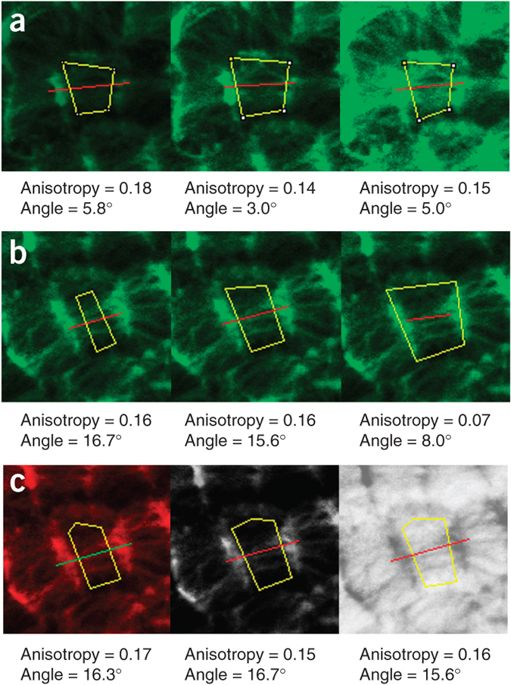
\includegraphics[scale=0.6]{imagenes/fibritool.jpg}
        \caption{\'Area de inter\'es seleccionada manualmente en amarillo, y resultado de FibriTool en rojo o verde. Fuente: \cite{boudaoud2014fibriltool}}
        \label{fig:fibritool}
\end{figure}

% Quantitative IFS
Otra investigaci\'on de extracci\'on e individualizaci\'on de filamentos es \cite{qiu2014quantitative}, la que propone un filtro de detecci\'on de caracter\'isticas de 6 pasos m\'as un algoritmo llamado \textit{SBDA} que busca eliminar segmentos de filamentos menores a 2 p\'ixeles (Figura \ref{fig:IFS}). 
\begin{figure}[H]
        \centering
        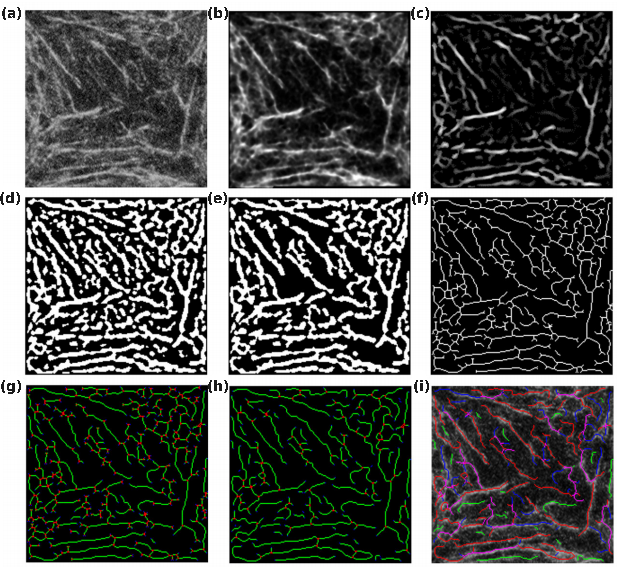
\includegraphics[scale=0.75]{imagenes/QuantitativeIFS.png}
        \caption{Etapas de individualizaci\'on de filamentos de \cite{qiu2014quantitative}. (A): Imagen de red de fibras de un osteoblasto .(B, C, D, E, F): Filtros de limpieza, tubularidad, segmentaci\'on, conectividad y esqueletonizaci\'on. (G): Clasificaci\'on topol\'ogica de intersecciones a nivel de pixel. (H): Resultado de algoritmo SBDA. (I): Individualizaci\'on de segmentos de filamentos seg\'un forma estructural: aislado (verde), solapado (morado) u otro (azul). Fuente: \cite{qiu2014quantitative}}
        \label{fig:IFS}
\end{figure}

%describir filtros, intensidad es con fibre coefficient
Las 6 etapas de filtro consideradas en este m\'etodo comienzan por reducir el ruido y realzar el contraste de la imagen, aumentando la intensidad de los p\'ixeles que est\'en sobre un umbral, al mismo tiempo que eliminan los p\'ixeles que se encuentren debajo del mismo umbral. El segundo paso consiste en filtrar informaci\'on estructural, que se basa en los eigenvalores de la matriz Hessiana, buscando descartar objetos en la imagen que no correspondan a una figura tubular. El tercer filtro ejecuta una limpieza sobre lo que se define como \textit{se\~nales d\'ebiles}, pudiendo ser estructuras con una intensidad baja y/o aisladas y por ende no corresponden a elementos en el plano focal de inter\'es. Finalmente, el filtro de esqueletonizaci\'on realiza un adelgazamiento de la imagen, en el que cada estructura pasa a tener 1 p\'ixel de ancho, facilitando el an\'alisis topol\'ogico posterior. \\

%describir SBDA, el analisis es a nivel de pixel
La clasificaci\'on topol\'ogica consiste en el an\'alisis a nivel de p\'ixel y su vecindario de 8 p\'ixeles alrededor para determinar si este corresponde a un punto aislado, al final de un fragmento de filamento, a un punto interior de un filamento, o a una junci\'on de filamentos. Seguido de aquello, el algoritmo SBDA realiza otro an\'alisis topol\'ogico a nivel de p\'ixel que borra los segmentos menores a 3 p\'ixeles, adem\'as de realizar los calculos de distancia de cada segmento/fragmento. Por último, se lleva a cabo una combinaci\'on de segmentos para construir los filamentos basandose en el par\'ametro $W$, llamado \textit{ancho efectivo}, cuyo valor define si la uni\'on de 2 o m\'as segmentos se trata de una bifurcaci\'on, una intersecci\'on o un sobrelapamiento. 

% se mide caracteristicas geometricas, como largo, distribucu\'on de la orientaci\'on, y como los resultados son afectados por el ruido.
Como resultados de \cite{qiu2014quantitative}, se obtienen caracter\'isticas geom\'etricas como el largo de los filamentos y la distribuci\'on de la orientaci\'on de los filamentos, as\'i como la variaci\'on de estos valores para variaciones en la relaci\'on entre la se\~nal y el ruido de la imagen.

%SOAX, extraccion y cuantifiacion de la red
Por su parte, la investigaci\'on de \cite{xu2015soax}, llamada SOAX, utiliza curvas param\'etricas de contorno abierto (SOAC en ingl\'es) en conjunto con una funci\'on de minimizaci\'on para obtener un peque\~no set de candidatos de soluciones \'optimas, de las que el usuario puede elegir una. Las curvas param\'etricas de contorno abierto son reguladas por 2 par\'ametros: $\tau$, que fija el umbral de intensidad desde el que se inicializa una SOAC, siendo los puntos de intensidad m\'aximos locales de la imagen. El segundo par\'ametro, $K_str$, es el factor que regula la elongaci\'on/evoluci\'on de cada SOAC. Una vez concluida la inicializacio\'on y evoluci\'on de curvas SOAC, se identifican las junciones/intersecciones generadas entre diversas curvas SOAC, agrup\'andose seg\'un su cercan\'ia.  

\begin{figure}[h]
        \centering
        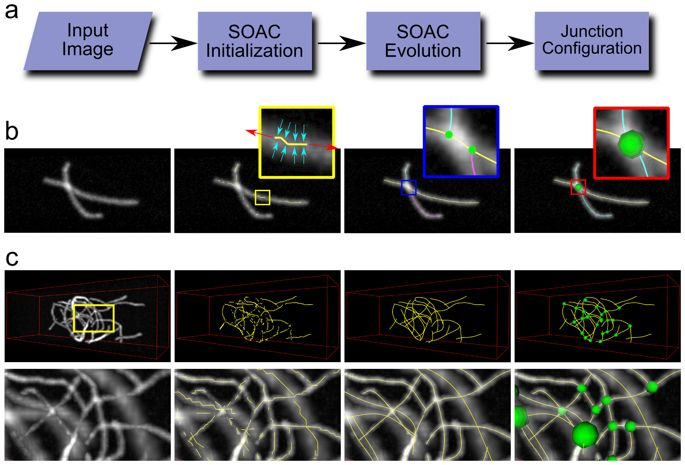
\includegraphics[scale=0.75]{imagenes/SOAX.jpg}
        \caption{Etapas de SOAX: A partir de los puntos de alta intensidad se inicializan curvas param\'etricas de contorno abierto (SOAC en ingl\'es), las que crecen, generando intersecciones entre ellas. Finalmente, se agrupan las intersecciones más cercanas. Fuente: \cite{xu2015soax}}
        \label{fig:SOAX}
\end{figure}

La funcio\'on de minimizaci\'on que los autores denominan como  \textit{F-Function}\eqref{eq:FFunction}, se encuentra definida por otros 2 par\'ametros: El factor $c$ ($c > 1$) que regula la penalizaci\'on de las SOACs con bajo \textit{Signal to Noise Ratio}, y el umbral $t$, que define bajo que n\'umero se considera como bajo el \textit{Signal to Noise Ratio}. El umbral $t$ se ve reflejado en $L_<t$ dentro de la \textit{F-Function}, como el largo de SOACs en una regi\'on de la imagen con \textit{Signal to Noise Ratio} por debajo de $t$.

\begin{equation}
   \label{eq:FFunction}
    F = -L_total + {c}{L_<t} 
\end{equation}

Para estos m\'etodos, se han indicado como cr\'iticas la dificultad para identificar correctamente un filamento de otro, en los casos de  superposici\'on, fragmentaci\'on, o variaciones de intensidad en la imagen.
% describir alguno de estos papers 

En la segunda categor\'ia, \cite{cerda2014geometrical} plantea la identificaci\'on de segmentos de filamentos como un problema de asignaci\'on, utilizando las medidas de distancia euclidiana y angular como restricciones, y el algoritmo h\'ungaro para su resoluci\'on. En la misma categor\'ia, \cite{breuer2015define} realiza la asociaci\'on de la red con un grafo no dirigido con pesos, en el que cada filamento es equivalente a un camino en el grafo. Esto permite que la b\'usqueda e individualizaci\'on de filamentos, con un segmento de filamento representado por una arista del grafo, sumado a las restricciones que plantea el autor, sea tratado como un problema de {\it Set Cover}. En el caso de los m\'etodos de la segunda categor\'ia, la mayor cr\'itica es su costo computacional alto, lo que limita en parte aquel enfoque. Se debe agregar que los par\'ametros utilizados por estas t\'ecnicas (\'angulos o  distancias m\'aximas entre filamentos) son complejas de obtener de los expertos directamente. Sin embargo, una de sus ventajas es que automatizan la recuperaci\'on de informaci\'on incluyendo una mayor cantidad de propiedades a cada arista. 


%En particular, el m\'etodo {\it FCP} presentado en la secci\'on \ref{Antecedentes}, utiliza s\'olo el grosor como caracter\'istica en la etapa de asignaci\'on de pesos a las aristas del grafo, lo que es usado en la funci\'on de minimizaci\'on del problema de optimizaci\'on planteado por ellos. En la etapa de selecci\'on del subconjunto de caminos, el mismo m\'etodo desarrolla una heur\'istica que utiliza {\it BFS} en conjunto con el \'angulo de deflexi\'on entre aristas. El mismo m\'etodo evita realizar un recorrido de grafos, al buscar las combinaciones de caminos del subconjunto P' que dan lugar a uno o m\'as filamentos mediante la minimizaci\'on de un {\it Set Cover}. 

%representa un camino en este grafo, y los conjuntos de caminos 
\medskip
%Todos estos enfoques, cuya entrada principal de datos son las im\'agenes etiquetadas a trav\'es de marcadores fluorescentes, 
% basados en grafos

A modo de ejemplo, el programa \texttt{DeFine} desarrollado en \cite{breuer2015define} describe el problema de identificaci\'on de filamentos como un problema de b\'usqueda de caminos, es decir, como un problema del tipo {\it Path Cover}. Se define el peso de cada segmento/arista por un c\'alculo de {\it aspereza}, asociada al grosor o intensidad de la arista o un conjunto de estas.
%, o tambi\'en puede ser calculado respecto al \'angulo entre aristas.
Este problema particular es llamado {\it Filament Covering Problem} (FCP) y los autores demuestran que es NP-Hard, por lo que proponen un algoritmo de aproximaci\'on mediante \textit{Set Cover}, cuyo objetivo es que cada arista pertenezca al menos a un conjunto. La definici\'on de {\it Set Cover} es:

\begin{quote}
Dado un conjunto de elementos, denominado universo, y $n$ conjuntos cuya unión comprende el universo, el {\it Set Cover Problem} consiste en identificar el menor n\'umero de conjuntos cuya unión a\'un contiene todos los elementos del universo.
\end{quote}

La adaptaci\'on a lo definido por {\it FCP} es: 
\begin{quote}
Sea el universo $U$ conformado por las aristas del grafo, y un conjunto $S$, conformado por conjuntos de aristas, cada uno con costo $c_s$, $s \in S$:

Encontrar un subconjunto $S_{set} \subseteq S$ con costo m\'inimo (o promedio, dependiendo de la forma en que se calcula la aspereza) tal que cada elemento en $U$ este cubierto al menos una vez.
\end{quote}

Con la demostraci\'on de que FCP es NP-Hard, dado que la cantidad de caminos crece de forma exponencial respecto al n\'umero de nodos, los autores de \cite{breuer2015define} plantean la elecci\'on de un subconjunto de caminos, con los que pueden expresar el problema de {\it Set Cover} como algoritmo de aproximaci\'on lineal fraccional binario. El subconjunto de caminos puede obtenerse con la heur\'istica de recorrer el grafo por su anchura ({\it Breadth-First Search}), deteni\'endose al momento que el \'angulo de deflexi\'on entre aristas adyacentes supere 60\degree, o de caminos generados a partir de 100 \'arboles de expansi\'on m\'inima aleatoria ({\it RMST}), aportando cada uno de los 100 con $N(N-1)/2$ caminos no triviales y sin direcci\'on. El flujo de decisiones para generar el subconjunto de caminos puede observarse en la figura \ref{fig:define-set-cover}.

\begin{figure*}[h!]
    \centering
    \label{fig:flujo-expected}
    \begin{subfigure}[t]{\textwidth}
        \centering
        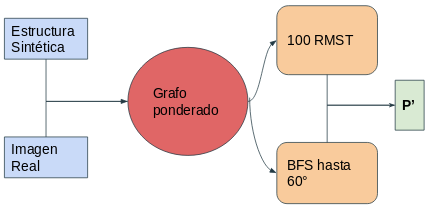
\includegraphics[scale=0.5]{imagenes/flujoDefine.png}
        \caption{Entrada de datos y elecci\'on de subconjunto de caminos {\bf P'} en DeFine.}
        \label{fig:define-set-cover}
    \end{subfigure}%
    \vskip\baselineskip
    \begin{subfigure}[t]{\textwidth}
        \centering
        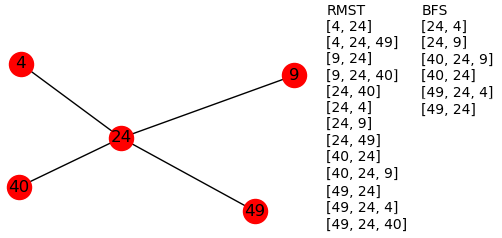
\includegraphics[scale=0.8]{imagenes/BFSvsRMSTpaths.png}
        \caption{Subconjunto {\bf P'} para el grafo de 5 nodos a la izquierda, utilizando la opci\'on de 100 {\it RMST} o heur\'istica de {\it BFS} que corta el camino al encontrar un \'angulo de deflexi\'on mayor a 60\degree entre aristas adyacentes.  }
        \label{fig:subconjunto-p-prima-caminos-posibles}
    \end{subfigure}
    \caption{(\ref{fig:define-set-cover}) A partir de un grafo ponderado proveniente de una estructura sint\'etica o de una imagen real, se elige {\bf P'} entre los $N(N-1)/2$ caminos no triviales y sin direcci\'on que aporta cada uno de los 100 \'arboles de expansi\'on m\'inima aleatoria ({\it RMST}), o los caminos resultantes de la heur\'istica de b\'usqueda por anchura ({\it BFS}) con interrupci\'on al dar con una arista que tenga un \'angulo superior a 60\degree. (\ref{fig:subconjunto-p-prima-caminos-posibles}) Subconjunto {\bf P'} de P, para el grafo de 5 nodos de ejemplo a la izquierda. }
    \end{figure*}
    
    
Este enfoque faculta que al tener un grafo que representa la red de filamentos, como en la figura \ref{Fig1d}, sea posible llegar a resultados como los que aparecen en las figuras \ref{Fig2a} o \ref{Fig2b} a trav\'es de la asignaci\'on de pesos a la aristas, y de restricciones a las uniones entre las mismas. Cabe destacar que el {\it FCP} s\'olo utiliza 2 caracter\'isticas independientes para describir los segmentos de los filamentos, siendo el \'angulo de deflexi\'on entre aristas usado en la etapa de selecci\'on de subconjuntos de caminos s\'olo si es seleccionada la heur\'istica {\it BFS}, y el grosor, empleado para describir el peso de las aristas.  
%es de complejidad $\mathcal{O}(N^{(2K+2)})$, con $N$ como n\'umero de nodos y $k$ como el n\'umero m\'aximo de caminos que pasan por cada v\'ertice. 
% Aquello permitir\'ia pasar de Fig1d a Fig2b por ejemplo

%\begin{defn}[ver \cite{KAR00}] Definición definitiva %$$\frac{d}{dx}\int_a^xf(y)dy=f(x).$$\end{defn}